%----------------------------------------------------------------------------
\chapter{Architektúra}
%----------------------------------------------------------------------------
Az alkalmazás 3 fő részre bontható frontend, backend valamint adatbázis.
E három réteg együttesen felel azért, hogy a felhasználó böngészőn keresztül érkező interrakcióit kezelje és az állapotot tárolja.
%----------------------------------------------------------------------------

\section{Adatbázis séma}
Az adatbázis migrációját nem kellett manuálisan végrehajtanom hála a Prisma-nak. 
A Prisma - amellett, hogy kezeli a migrációkat - egy absztrakciós réteget ad az adatbázisunk és az alkalmazásunk közé olyan szinten, hogy teljesen elfedi az adatbázist a fejlesztő elöl.

Ennek ellenére mégis relációs adatbázist terveztem, majd ezt ültettem át a Prisma által kíván sémába.
Tanulmányaim során ezzel a tervezési metodikával találkoztam és olyannyira rögzült, hogy elöszőr nehéz volt kicsit más szemszögből vizsgálni a problémát.

\begin{figure}[!ht]
  \centering
  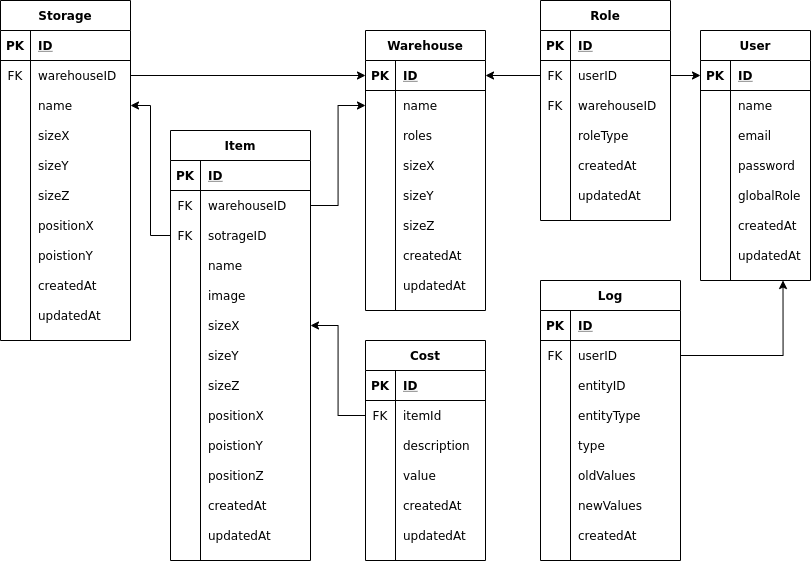
\includegraphics[width=150mm, keepaspectratio]{figures/db.png}
  \caption{Adatbázis séma}
  \label{fig:backend}
\end{figure}

%----------------------------------------------------------------------------

\section{Backend felépítése}
Az alkalmazás üzleti logikáját megvalósító rész egy NodeJS-re épülő rendszer.
Az alkalmazás egyetlen egy végpontot ajánl a kliensek számára.
A kéréseket egy express server fogadja, a feldolgozásának mikéntjéről pedig egy Apollo server gondoskodik, itt történik meg a GraphQL elemzése és ez alapján a megfelelő kódrészlet futtatása.
Az Apollo server lehetőséget nyújt middelware-ek definiálsára, melyek minden kérés kiszolgálása elött lefutnak.
Erre a lehetőségre épít a GraphQL Shield nevű könyvtár, aminek segítségével minden egyes GraphQL műveletre megadhatünk ahhoz szükséges előfeltételeket egyszerű szabályok segítségével.
Ilyen szabályokkal valósítottam meg a teljes authorizációt és az authentikáció ellenörzését is.

\begin{figure}[!ht]
  \centering
  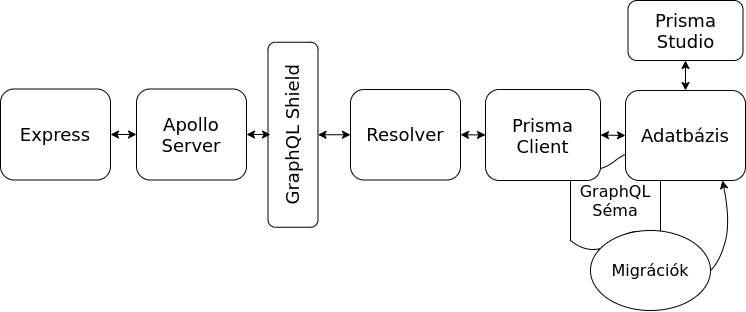
\includegraphics[width=150mm, keepaspectratio]{figures/backend.png}
  \caption{Backend felépítése}
  \label{fig:backend}
\end{figure}

A megfelelő kódrészlet és a middelware-ek futtatása után, a Prismán keresztül az adatbázishoz fordulunk adat lekérés vagy modósítás miatt.

Az ábrán (\refstruc{fig:backend}) világosan látszik, hogy a Prisma által nyújtott studio az adatbázishoz csatlakozik, így az általunk írt üzleti logika nem fog érvenyesülni.
Fontos, hogy az itt végrehajtott modósítások nem várt működéshez is vezethetnek.

%----------------------------------------------------------------------------

\section{Frontend felépítése}

\begin{figure}[!ht]
  \centering
  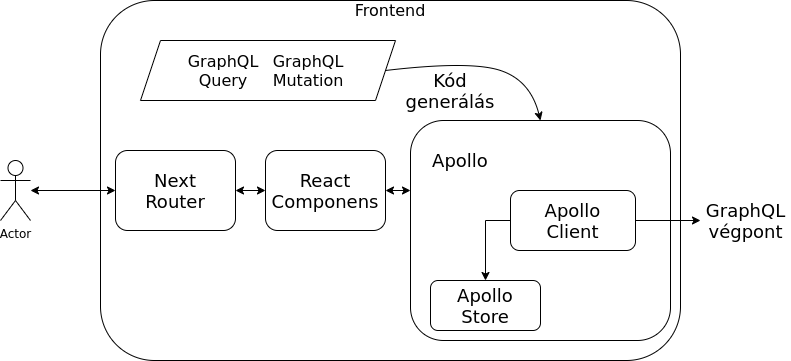
\includegraphics[width=150mm, keepaspectratio]{figures/frontend.png}
  \caption{Frontend felépítése}
  \label{fig:frontend}
\end{figure}

Ahogy azt a korábbi fejezetekben taglaltam a kliens alkalmazás megvalósításához React-et azon belül pedig NextJS-t használtam.
A backendhez csatlakozást az Apollo Client könyvtárral oldottam meg. 
Az Apollo Client és az Apollo Server együtt egy nagyon jól és könnyen használható rendszert alkotnak.
A Client megkapja a Server-től a GraphQL sémát, így fejlesztés közben kódkiegészítéssel és tipus ellenörzéssel írhatjuk a lekérdezéseinket.
Ezen felül lehetőségünk nyílik kódgenerálásra is.
A megírt GraphQL Query és GraphQL Mutation kódokból React hook-okat kapunk, melyekben az állapot- és a típusokkezelés is megvalósított

%----------------------------------------------------------------------------

\section{Architektúra összefoglalása}
Tehát a három fő komponense az alkalmazásnak a frontend, a backend és az adatbázis.
A frontend és a backend közötti kommunikáció GraphQL segítségével történik az Apollo Cliens és az Apollo Server között.
A backend és az adatbázis kommunikációja pedig SQL segítségével történik, azonban ezt a Prisma teljesen elfedi.

\begin{figure}[!ht]
  \centering
  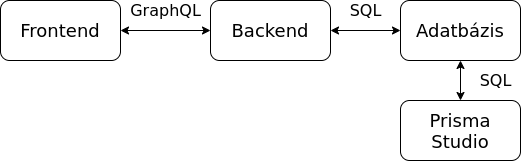
\includegraphics[width=150mm, keepaspectratio]{figures/architecture.png}
  \caption{Teljes alkalmazás felépítése}
  \label{fig:architecture}
\end{figure}